\documentclass[a4paper, titlepage]{jsarticle}

\date{\today}
\usepackage[dvipdfmx]{graphicx}
\usepackage{url}
% \usepackage[T1]{fontenc}
\usepackage{float}
\usepackage{ascmac}
\usepackage{pdfpages}
\usepackage{enumitem}
\usepackage{otf}
\usepackage{morefloats}
% \usepackage{morefloats}
\usepackage{comment}


\newcommand{\system}{\textsl{Aero Net}}
\maxdeadcycles=10000
\begin{document}
\begin{titlepage}
  \centering
  \vspace*{150truept}
  {\Large 外部設計書}\\
  \vspace*{50truept}
  {\Huge ドローン宅配事業者支援システム} \\
  \vspace{15truept}
  {\Huge \system} \\
  \vspace{50truept}
  {\LARGE 土佐山田IT株式会社}\\
  \vspace{20truept}
  {\large{\tabcolsep = 1cm
      \begin{tabular}{ccc}
        久保田 天治 & 塩澤 康志 & 蝉 祐介  \\
        寺内 俊輔  & 林 晃太郎 & 松本 吏司
      \end{tabular}
    }}
\end{titlepage}
% \fig{filename(.pdf無し)}
% \newcommand{\fig}[1]{
%   \begin{figure}[H]
%     \centering
%     \includegraphics[width=\linewidth]{pdf/#1.pdf}
%     \caption{#1}
%     \label{fig:#1}
%   \end{figure}
% }
% \fig{filename(.pdf無し)}{caption}
\newcommand{\fig}[2]{
  \begin{figure}[H]
    \centering
    \includegraphics[width=\linewidth]{flow/#1.pdf}
    \caption{#2}
    \label{fig:#1}
  \end{figure}
  \clearpage
}
\newcommand{\ui}[2]{
  \begin{figure}[H]
    \centering
    \fbox{
      \includegraphics[width=0.65\textwidth]{ui/#1}
      }
    \caption{#2}
    \label{fig:#1}
  \end{figure}
}

\tableofcontents

\clearpage

\section{システム化の背景・目的}
2022年日本における宅配便取扱個数は50億個を超えた
図\ref{fig:number}のように宅配需要は近年増加し続けている,しかし,宅配サービスの拡大と需要増加には新たな課題も浮かび上がっている.
最も顕著な課題は宅配業界における労働力不足だ.図\ref{fig:driver}のように道路貨物運送業の自動車運転者は減少を続けている.
この問題を解決するためにより効率的な配送方法が必要である.

ドローン宅配事業者支援システム\system の目的は,宅配業界の労働力不足の問題を自動運転で運用するドローンを用いることで解決することである.
そのためには多くの事業者にドローン宅配を利用してもらうため,ドローン宅配事業者を支援するためのベースとなるサービスを制作する.
このシステムを導入することにより,今後日本国内で増加するであろう宅配便取扱個数の増加と労働力不足を宅配業界全体で乗り越えられると考える.
%aaa
\begin{figure}[H]
  \centering
  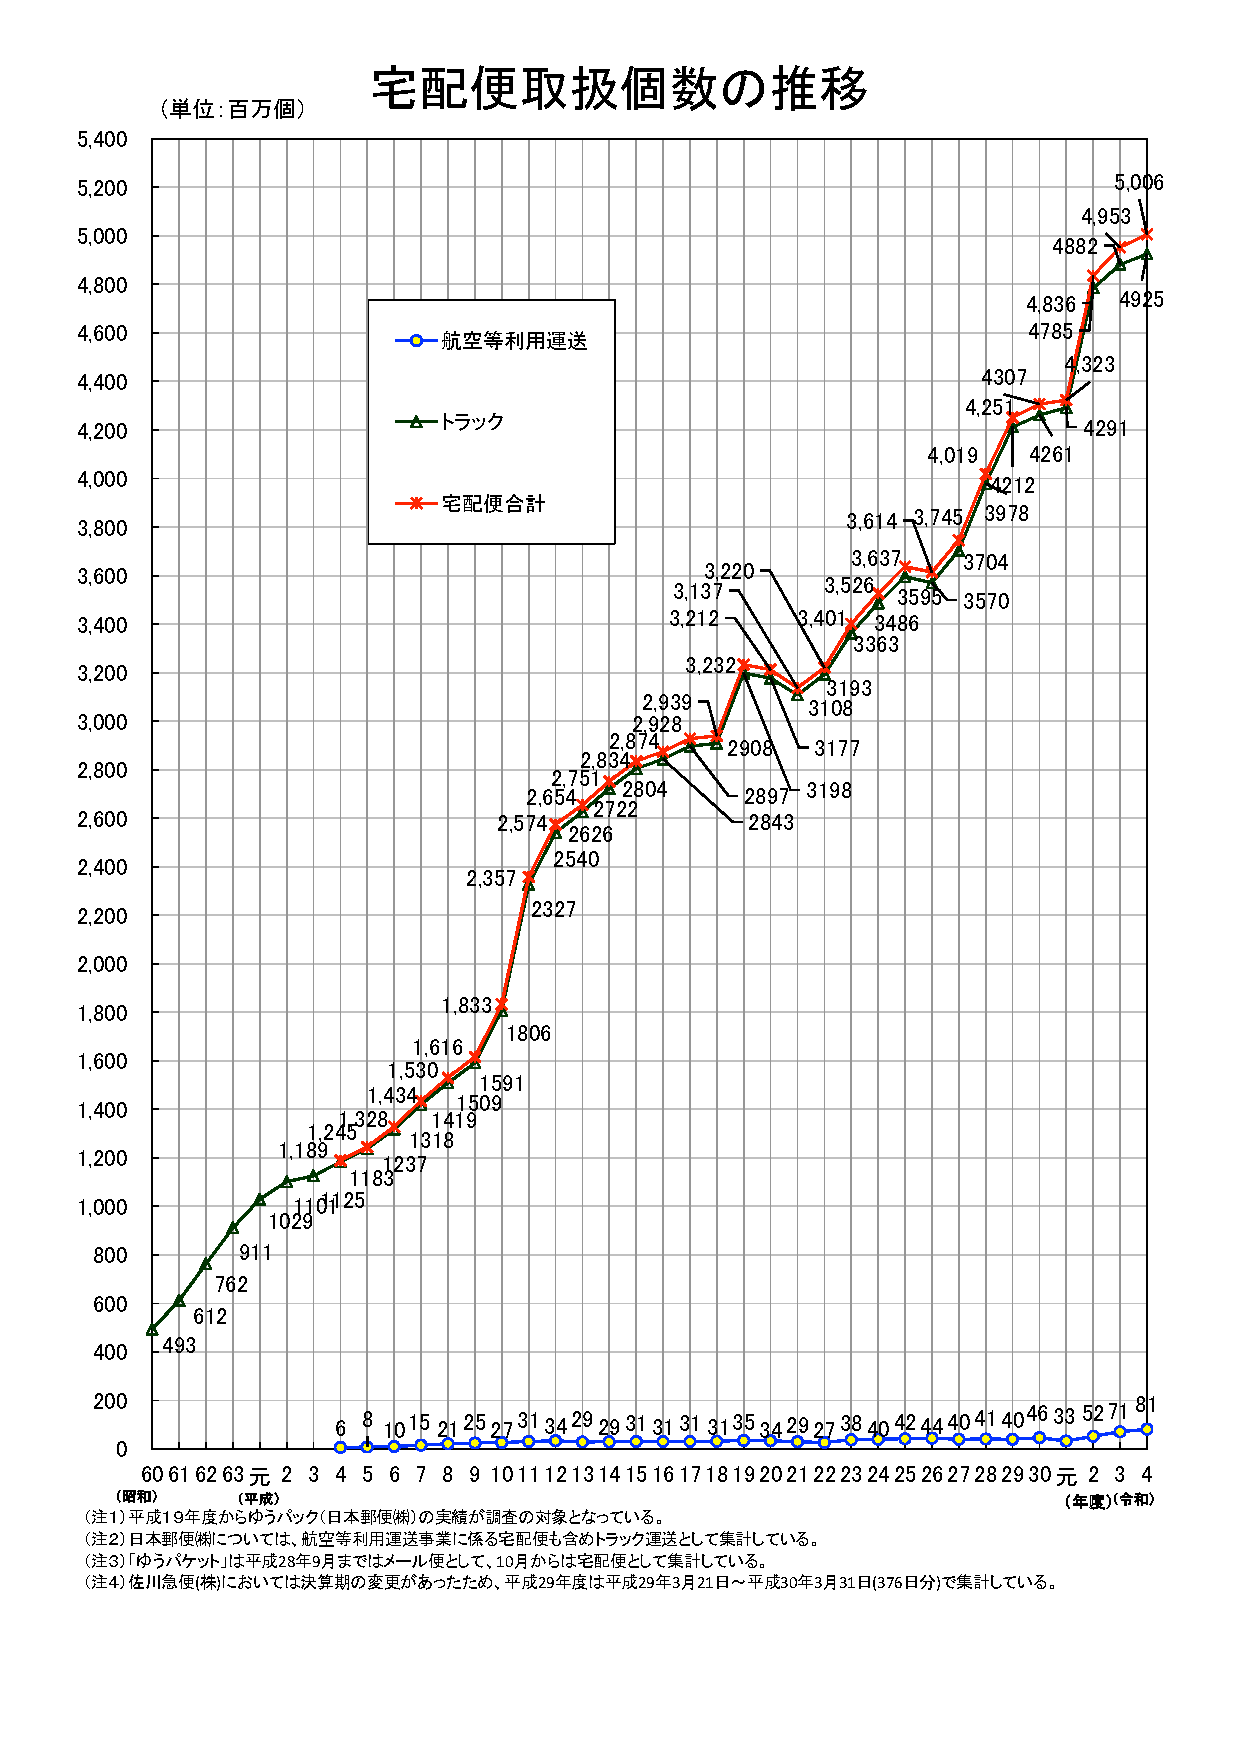
\includegraphics[height=0.8\textheight]{other/number.pdf}
  \caption{年間宅配便取扱個数(\cite{home_delivery_2022}より引用)}
  \label{fig:number}
\end{figure}
\begin{figure}[H]
  \centering
  \includegraphics[width=\textwidth]{other/driver2.pdf}
  \caption{道路貨物運送業の自動車運転者(\cite{Human_Resource}より引用)}
  \label{fig:driver}
\end{figure}

% \section{業務フロー図}
%流れ.
\section{機能設計}
本システムは管理者,事業者,利用者が存在する.それぞれに向けた機能設計を記述する.
\clearpage
\subsection{管理者向け機能}
管理者用のwebページを作成し下記の機能を設ける.
\begin{description}[labelwidth=\linewidth]
  \setlength{\leftskip}{1em}

  \item [ログイン機能] 管理者がユーザ名,パスワード入力フィールドに情報を入力することでログインすることができ,
  ログイン状態を保持できる機能である.入力内容が正しい場合,ログイン状態になあり,トップページに遷移する.
  \fig{admin_login}{ログイン機能}
  \item [ログアウト機能] 本システムにログインしている管理者が,ログイン状態を解除できる機能.
  ログアウトするとログイン画面に遷移する.
  \fig{admin_logout}{ログアウト機能}



  % \item [事業者管理機能] 事業者の登録情報の管理閲覧,絞り込み,請求書の送付,支払い状態の管理閲覧,貸与ドローンの管理閲覧する機能.
  % 登録情報管理ボタン,支払い状態管理ボタン,貸与ドローン管理ボタンでそれぞれ対応したページ(登録情報詳細,支払い状態詳細,貸与ドローン詳細)に遷移する.
  % 左にあるチェックボックスを選択して,一括請求書の送付ボタンで一括で請求書を送付できる.各種データでソートと絞り込みを行えるようにする.
  % 全選択,チェックに一括請求書送付ボタン,絞り込みボタン.
  % チェックボックス,事業者名,事業拠点数,登録住所の都道府県,貸与ドローン数,直近7日間の宅配実績,支払い実績,請求書の送付,登録情報管理ボタン,支払い状態管理ボタン,貸与ドローン管理ボタンが並んでいる.
  % 一画面に収める.
  % (登録情報,支払い状態,貸与ドローン情報は基本的に自動で更新されるが,手動操作も可能にしている)
  \item [事業者一覧閲覧機能] 事業者の一覧を表示閲覧する機能,この機能で表示する事業者一覧から事業者に対する各種操作を行う.
  \fig{admin_view_coop_list}{事業者一覧閲覧機能}
  \item [事業者絞り込み機能] 事業者の一覧から条件により絞り込みを行う機能.
  \fig{admin_filter_coop}{事業者絞り込み機能}
  \item [事業者検索機能] 事業者の一覧から条件により検索を行い,検索結果を表示する機能.
  \fig{admin_search_coop}{事業者検索機能}
  \item [情報並び替え機能] 事業者の一覧からある項目を用いて並べ替えを行う機能.
  \fig{admin_sort_coop_info}{情報並び替え機能}
  \item [請求書送付機能] 事業者に対してメールで請求書を送付する機能.
  \fig{admin_send_coop_bill}{請求書送付機能}
  \item [事業者情報詳細閲覧機能] 選択した事業者の詳細情報を表示する機能.
  \fig{admin_view_coop_info}{事業者情報閲覧機能}
  \item [事業者情報編集機能] 選択した事業者の情報を編集する機能.
  \fig{admin_edit_coop_info}{事業者情報編集機能}
  \item [事業者支払い情報詳細閲覧機能] 事業者の支払い情報の詳細を閲覧する機能.
  \fig{admin_view_coop_pay_info}{事業者支払い情報閲覧機能}
  \item [事業者支払い情報詳細編集機能] 事業者の支払い情報を編集する機能.
  \fig{admin_edit_coop_pay_info}{事業者支払い情報編集機能}
  \item [事業者ドローン情報詳細機能] 事業者のドローン情報の詳細を閲覧する機能.
  \fig{admin_view_coop_drone_info}{事業者ドローン情報閲覧機能}
  \item [事業者ドローン情報編集機能] 事業者のドローン情報を編集する機能.
  \fig{admin_edit_coop_drone_info}{事業者ドローン情報編集機能}

  % \begin{figure}[H]
  %   \centering
  %   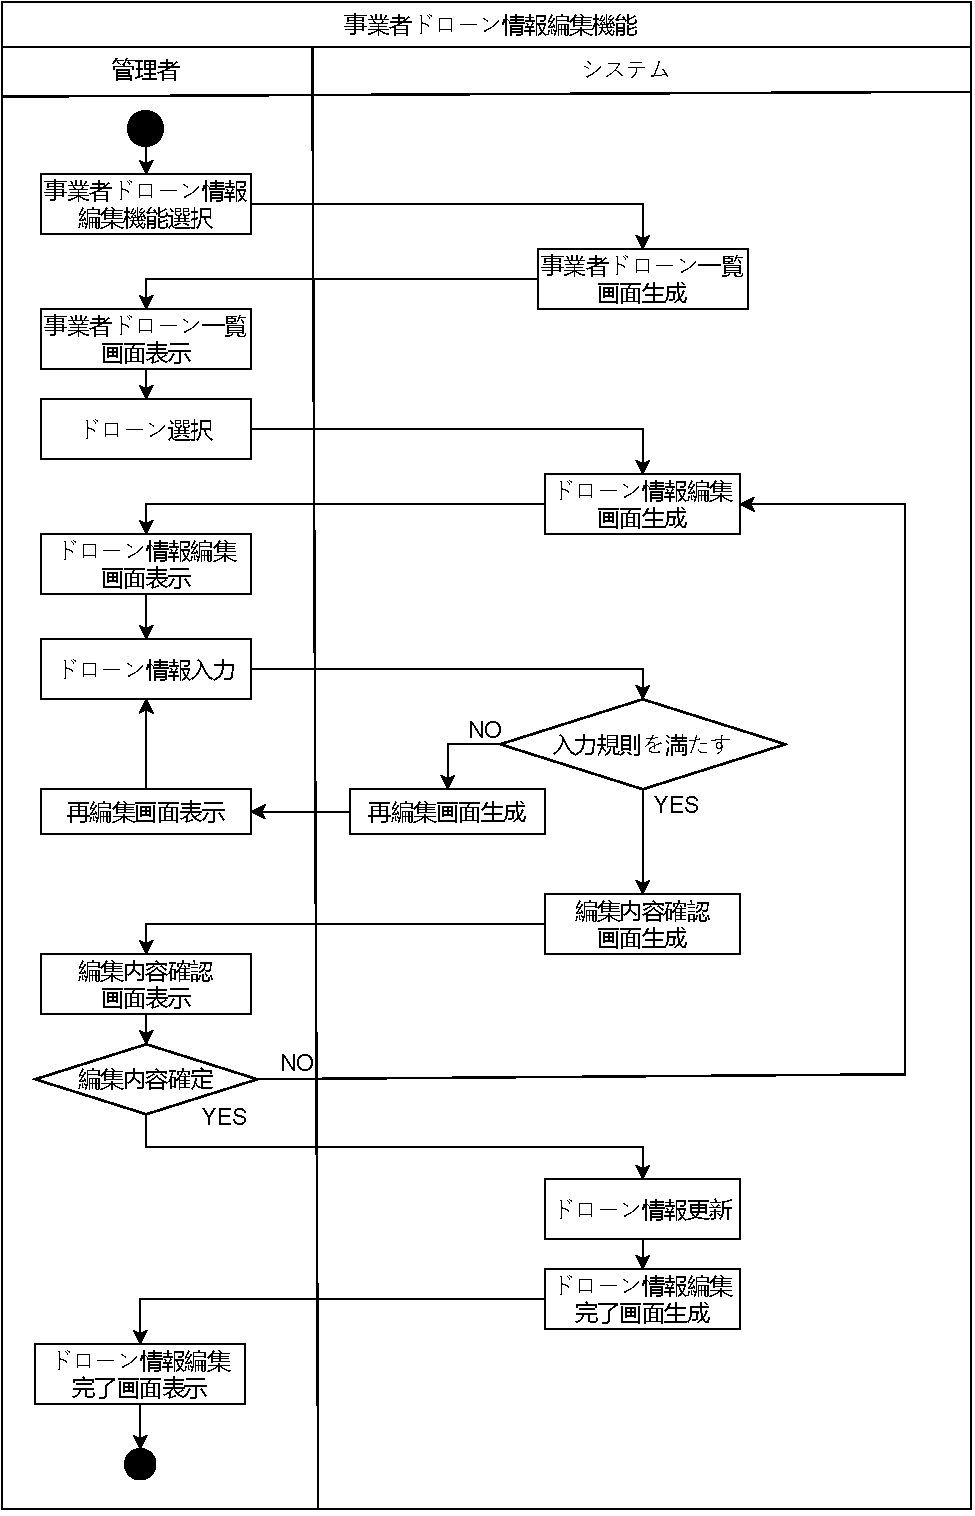
\includegraphics[width=0.8\textwidth]{flow/drone_info_editor.pdf}
  %   \caption{事業者ドローン情報編集機能}
  %   \label{fig:drone_info_editor}
  % \end{figure}



  % \item [利用者管理機能] 利用者の登録情報の管理閲覧,絞り込み,請求書の送付,支払い状態の管理閲覧する機能.
  % 登録情報管理ボタン,支払い状態管理ボタンでそれぞれ対応したページに遷移する.各種データでソートと絞り込みを行えるようにする.
  % 大体上と同じ.
  % (先払いを前提にすることで請求書送付機能いらない気がしてきた)
  \item [利用者一覧閲覧機能] 利用者の一覧を表示閲覧する機能,この機能で表示する利用者一覧から利用者に対する各種操作を行う.
  \fig{admin_view_user_list}{利用者一覧閲覧機能}
  \item [利用者絞り込み機能] 利用者の一覧から条件により絞り込みを行う機能.
  \fig{admin_filter_user}{利用者絞り込み機能}
  \item [利用者検索機能] 利用者の一覧から条件により検索を行い,検索結果を表示する機能.
  \fig{admin_search_user}{利用者検索機能}
  \item [情報並び替え機能] 利用者の一覧からある項目を用いて並べ替えを行う機能.
  \fig{admin_sort_user_info}{情報並び替え機能}
  \item [請求書送付機能] 利用者に対してメールで請求書を送付する機能.
  \fig{admin_send_user_bill}{請求書送付機能}
  \item [利用者情報詳細閲覧機能] 選択した利用者の詳細情報を表示する機能.
  \fig{admin_view_user_info}{利用者情報閲覧機能}
  \item [利用者情報編集機能] 選択した利用者の情報を編集する機能.
  \fig{admin_edit_user_info}{利用者情報編集機能}
  \item [利用者支払い情報詳細閲覧機能] 利用者の支払い情報の詳細を閲覧する機能.
  \fig{admin_view_user_pay_info}{利用者支払い情報閲覧機能}
  \item [利用者支払い情報詳細編集機能] 利用者の支払い情報を編集する機能.
  \fig{admin_edit_user_pay_info}{利用者支払い情報編集機能}



  \item [事業者統計情報表示機能] 事業者の統計情報表示機能.
  \fig{admin_view_coop_statistics_info}{事業者統計情報閲覧機能}
  \item [事業者情報絞り込み機能] 事業者の統計情報を絞り込む機能.
  \fig{admin_filter_coop_statistics_info}{事業者情報絞り込み機能}
  \item [事業者情報グラフ表示機能] 事業者情報のグラフを表示する機能.
  \fig{admin_view_coop_statistics_info_graph}{事業者情報グラフ閲覧機能}


  \item [利用者統計情報表示機能] 利用者の統計情報表示機能.
  \fig{admin_view_user_statistics_info}{利用者統計情報閲覧機能}
  \item [利用者情報絞り込み機能] 利用者の統計情報を絞り込む機能.
  \fig{admin_filter_user_statistics_info}{利用者情報絞り込み機能}
  \item [利用者情報グラフ表示機能] 利用者情報のグラフを表示する機能.
  \fig{admin_view_user_statistics_info_graph}{利用者情報グラフ閲覧機能}



  \item [宅配依頼一覧表示機能] 宅配依頼一覧を表示する機能.
  \fig{admin_view_user_delivery_request_list}{宅配依頼一覧閲覧機能}
  \item [絞り込み機能] 宅配依頼の絞り込みを行う機能.
  \fig{admin_filter_user_delivery_request}{絞り込み機能}
  \item [検索機能] 宅配依頼の検索を行う機能.
  \fig{admin_search_user_delivery_request}{検索機能}
  \item [情報ソート機能] 宅配依頼一覧のソートを行う機能.
  \fig{admin_sort_user_delivery_request}{情報ソート機能}




  % 各種データでソートと絞り込みを行えるようにする.
  % 上に,一括選択ボタン,一括貸出ボタン,一括拒否ボタン,絞り込みが並んでいる.
  % チェックボックス,事業者名,要求ドローンの型番,要求個数,貸出ボタン,拒否ボタンが並んでいる.
  % ボタンは確認が入る.

  \item [宅配仕事割り振り機能] 宅配依頼受付機能で呼び出す,事業者に仕事を割り振る機能.集配に向かう事業者と仲介トラックと最終的に配送する事業者の組み合わせを選ぶ.(基本的には自動で全部行う,動かなくなったらエラーを返す)
  \fig{admin_allocate_user_delivery_task}{宅配業務割り振り機能}
  \item [ドローン貸与申請一覧機能] ドローン貸与申請の一覧を表示する機能.
  \fig{admin_view_user_apply_drone_lend_list}{ドローン貸与申請一覧閲覧機能}
  \item [ドローン貸与機能] 事業者からドローン貸与申請を受けて貸出あるいは,申請の差し戻しを行う機能.
  \fig{admin_approve_user_delivery_task_allocate_drone_lend}{ドローン貸与承認機能}
  \item [絞り込み機能] 一覧の絞り込みを行う機能.
  \fig{admin_filter_user_delivery_task_allocate}{絞り込み機能}
  \item [検索機能] 検索を行う機能.
  \fig{admin_search_user_delivery_task_allocate}{検索機能}
  \item [情報ソート機能] 情報のソートを行う機能.
  \fig{admin_sort_user_delivery_task_allocate_info}{情報ソート機能}
  % \item [事業者ドローン情報一覧表示機能] 事業者ドローン情報の一覧を表示する機能.
  % \fig{}{事業者保有ドローン一覧閲覧機能}
  \item [絞り込み機能] 一覧の絞り込みを行う機能.
  \fig{admin_filter_coop_drone}{絞り込み機能}
  \item [検索機能] 検索を行う機能.
  \fig{admin_search_drone}{検索機能}
  \item [情報ソート機能] 情報のソートを行う機能.
  \fig{admin_sort_coop_drone_info}{情報ソート機能}
  \item [事業者ドローン情報編集] ドローンの各種詳細情報を表示する機能.
  \fig{admin_edit_coop_drone}{編集機能}
  \item [ドローン登録機能] ドローンを登録する機能.
  \fig{admin_register_coop_drone}{ドローン登録機能}
\end{description}




\subsection{事業者向け機能}
事業者用のwebページを作成し下記の機能を設ける.
\begin{description}[labelwidth=\linewidth]
  \setlength{\leftskip}{1em}

  \item [ログイン機能]  事業者がユーザ名,パスワード入力フィールドに情報を入力することでログインすることができ,
  ログイン状態を保持できる機能である.入力内容が正しい場合,ログイン状態になあり,トップページに遷移する.
  \fig{coop_login}{ログイン機能}
  \item [ログアウト機能]  本システムにログインしている事業者が,ログイン状態を解除できる機能である.
  ログアウトするとTOP画面に遷移する.
  \fig{coop_logout}{ログアウト機能}
  \item [事業者登録申請機能]  事業者名,事業代表者,免許情報,口座情報,事業拠点,従業員数,電話番号,メールアドレス,施設情報,パスワードを入力して事業者登録申請を行う機能.
  \fig{coop_apply_coop_register}{事業者登録申請機能}
  \item [事業者情報編集機能]  事業者名,事業代表者,免許情報,口座情報,事業拠点,従業員数,電話番号,メールアドレス,施設情報,パスワードを編集する機能.
  \fig{coop_edit_coop_info}{事業者情報編集機能}


  \item [絞り込み機能] 一覧の絞り込みを行う機能.
  \fig{coop_filter_user_delivery_request_list_view}{絞り込み機能}
  \item [検索機能] 検索を行う機能.
  \fig{coop_search_user_delivery_request_list_view}{検索機能}
  \item [情報ソート機能] 情報のソートを行う機能.
  \fig{coop_sort_user_delivery_request_list_view_info}{情報ソート機能}
  % \fig{coop_check_user_delivery_request_list_view_execute}{実行確認機能}
  \item [配達完了通知機能]  宅配が完了した場合に利用者に通知する機能.
  \fig{coop_notice_user_delivery_request_list_view_delivery_complete}{配達完了通知機能}
  \item [使用ドローン登録機能]  事業者が独自に購入したドローンを登録する機能.
  \fig{coop_register_user_delivery_request_list_view_use_drone}{使用ドローン登録機能}

  % \item [配達依頼一覧表示機能] 一覧を表示する機能.
  % \item [依頼受注判断機能]  管理者から送られる宅配依頼を承諾もしくは拒否する機能.
  % (宅配依頼全体ではなく,都道府県単位に分割されたもの)
  % 上に一括チェック,絞り込み,チェックの全承諾,チェックの全拒否ボタン.
  % 受け取り住所,届ける住所,報酬,依頼日時,承諾,拒否.
  % 承諾もしくは拒否する場合,確認の画面を一度挟む,その後にooしましたのポップアップを出す.
  % 画面遷移はしない.
  % 受けている宅配依頼の一覧画面から配達完了通知を出す.
  % 上に絞り込み.
  % 受け取り住所,届ける住所,報酬,依頼日時,配達状態,配達完了通知ボタン.
  % 配達完了通知ボタンを押した場合,確認が出てyesを押すと相手に配達完了通知が行く.
  % ドローンの着地と合わせて自動で切り替わるようにもしたい.
  % ドローンの型番,現状の使用時間,保険の有無,航続距離(必要があれば),台数を入力してドローンを一括で登録する.


  % \fig{view_child_accounts}{子アカウント一覧表示機能}
  % \item [絞り込み機能] 一覧の絞り込みを行う機能.
  % \fig{business_childAccountListViewFilter}{絞り込み機能}
  % \item [検索機能] 検索を行う機能.
  % \fig{business_childAccountListViewSearch}{検索機能}
  % \item [情報ソート機能] 情報のソートを行う機能.
  % \fig{coop_child_account_list_sort}{情報ソート機能}
  % % \item [一括選択機能] 一括選択をする機能.
  % % \fig{coop_all_select_child}{一括選択機能}
  % \item [一括実行機能] 選択したの機能を一括で実行する機能.
  % \fig{coop_all_do_child}{一括実行機能}
  % \item [子アカウント管理機能]  事業者が子アカウント発行機能を用いて発行した子アカウントの管理を行う機能.
  % 発行した子アカウントの一覧画面で管理を行う.
  % 上に新規アカウント発行,全チェック,絞り込み,プルダウンでチェック全ての(権限変更,パスワード再発行,削除),プルダウンで選んだ処理の実行ボタン.
  % id,メールアドレス,権限一覧,権限変更,パスワード再発行ボタン,削除ボタン.
  % ボタンを押した場合確認が出て,処理が終わったら同じ画面に戻る.
  % 新規アカウント発行は.

  \item [子アカウント一覧表示機能] 一覧を表示する機能.
  \fig{coop_view_child_coop_account_list}{子アカウント一覧閲覧機能}
  \item [子アカウント発行機能] 権限を限定した一般従業員用アカウントを発行して,同一事業者内で複数人が事業を行えるようにする機能.
  \fig{coop_publish_child_coop_account}{子アカウント発行機能}
  \item [子アカウント削除機能] 子アカウントの削除を行う機能.
  \fig{coop_delete_child_coop_account}{子アカウント削除機能}
  \item [子アカウント編集機能] 子アカウントの編集を行う機能.
  \fig{coop_edit_child_coop_account}{子アカウント編集機能}

  % 各種機能のチェックボックス画面から与える権限を選び,次へを押す.
  % 次の画面で登録用のメールアドレスとパスワード2回の入力を行うと発行ボタンを押せる.
  % あとは登録したメールアドレスに招待リンクが飛ぶ.


  \item [ドローン種類一覧機能] ドローンの種類を一覧表示する機能ここから,ドローンの貸与申請を行う.
  \fig{coop_view_admin_drone_lend_apply_types_list}{ドローン種類一覧閲覧機能}
  \item [ドローンの修理依頼機能] ドローンの修理を依頼する機能.
  \fig{coop_request_admin_drone_lend_apply_fix}{ドローンの修理依頼機能}
  \item [ドローンの機体トラブル報告] ドローンの機体に関するトラブルを管理者に報告する機能.
  \fig{coop_report_admin_drone_lend_apply_trouble}{ドローンの機体トラブル報告機能}
  \item [ドローン貸与申請機能] ドローン貸与の申請,ドローンの返却,ドローンの修理依頼,ドローンの機体トラブル報告をする機能.
  \fig{coop_apply_admin_drone_lend}{ドローン貸与申請機能}
  \item [退会機能] 事業を終了し,データ削除を申請して退会する機能.
  \fig{coop_withdraw}{退会機能}
  \item [所持ドローン一覧機能] 所持ドローンを一覧表示する機能.
  \fig{coop_view_own_drone}{所持ドローン一覧機能}

\end{description}




\subsection{利用者向け機能}
利用者向けのスマートフォン用ソフトウェアを用意し下記の機能を設ける.
\begin{description}[labelwidth=\linewidth]
  \setlength{\leftskip}{1em}

  \item [ログイン機能] 利用者がユーザ名,パスワード入力フィールドに情報を入力することでログインすることができ,
  ログイン状態を保持できる機能である.%入力内容が正しい場合,ログイン状態になあり,トップページに遷移する.
  \fig{user_login}{ログイン機能}
  \item [ログアウト機能] 本システムにログインしている利用者が,ログイン状態を解除できる機能である.
  \fig{user_logout}{ログアウト機能}
  \item [利用者会員登録機能] 利用者名,住所,電話番号,メールアドレス,パスワードを用いて利用者が会員登録をする機能,これは管理者の許可が必要ない.
  \fig{user_register_account}{利用者会員登録機能}
  \item [利用者会員情報編集機能] 利用者名,住所,電話番号,メールアドレス,パスワードを編集する機能.
  \fig{user_edit_info}{利用者会員情報編集機能}
  \item [宅配場所登録機能] 宅配で離着陸する場所を指定して登録編集する機能,外の画像を送信して申請をする.
  登録申請をしました画面を出す.
  \fig{user_apply_user_delivery_place}{宅配場所申請機能}
  \item [宅配依頼機能] 管理者に対して宅配を依頼する機能.
  \fig{user_request_delivery}{宅配依頼機能}
  \item [お気に入り一覧表示機能] お気に入り登録した相手を一覧表示する機能.
  \fig{user_view_favorites}{お気に入り一覧閲覧機能}
  \item [お気に入りからデータ参照機能] お気に入りからデータを取得して反映する機能.
  \fig{user_refer_favorites_data}{お気に入りからデータ参照機能}
  \item [受け取り完了通知機能] 受け取り完了を通知する機能.
  \fig{user_receive_notice_complete_delivery}{受け取り完了通知機能}
  \item [お気に入り登録機能] 配送相手をお気に入り登録する機能,これを用いて簡単に宅配を依頼する機能.
  \fig{user_register_favorites}{お気に入り登録機能}
  \item [退会機能] データ削除を申請して退会する機能.
  \fig{user_withdraw}{退会機能}
\end{description}


\section{ユーザインタフェース設計}
\subsection{画面遷移図}
管理者用ソフトウェアの画面遷移図は図\ref{fig:admin_diagram}であり,
事業者用ソフトウェアの画面遷移図は図\ref{fig:coop_diagram},
利用者用ソフトウェアの画面遷移図は図\ref{fig:user_diagram}である.

\begin{figure}[H]
  \centering
  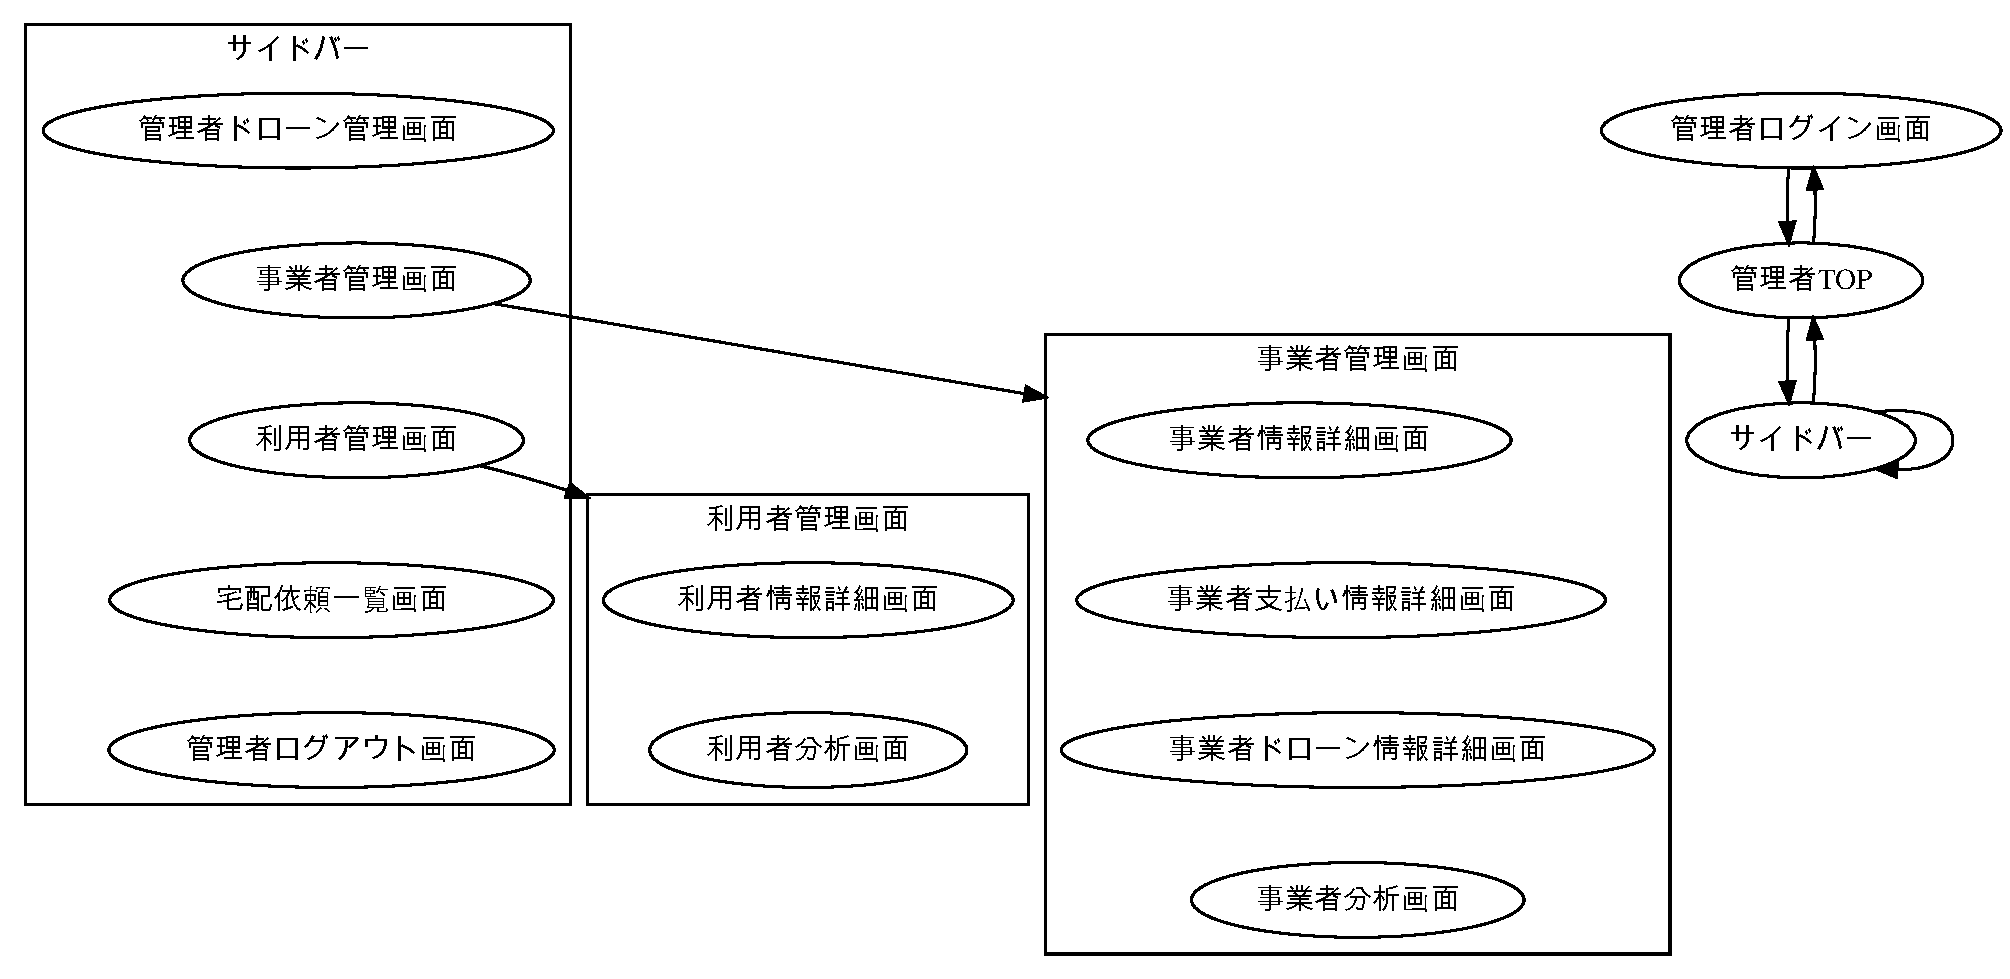
\includegraphics[width=\linewidth]{other/admin.pdf}
  \caption{管理者用ソフトフェアの画面遷移図}
  \label{fig:admin_diagram}
\end{figure}

\begin{figure}[H]
  \centering
  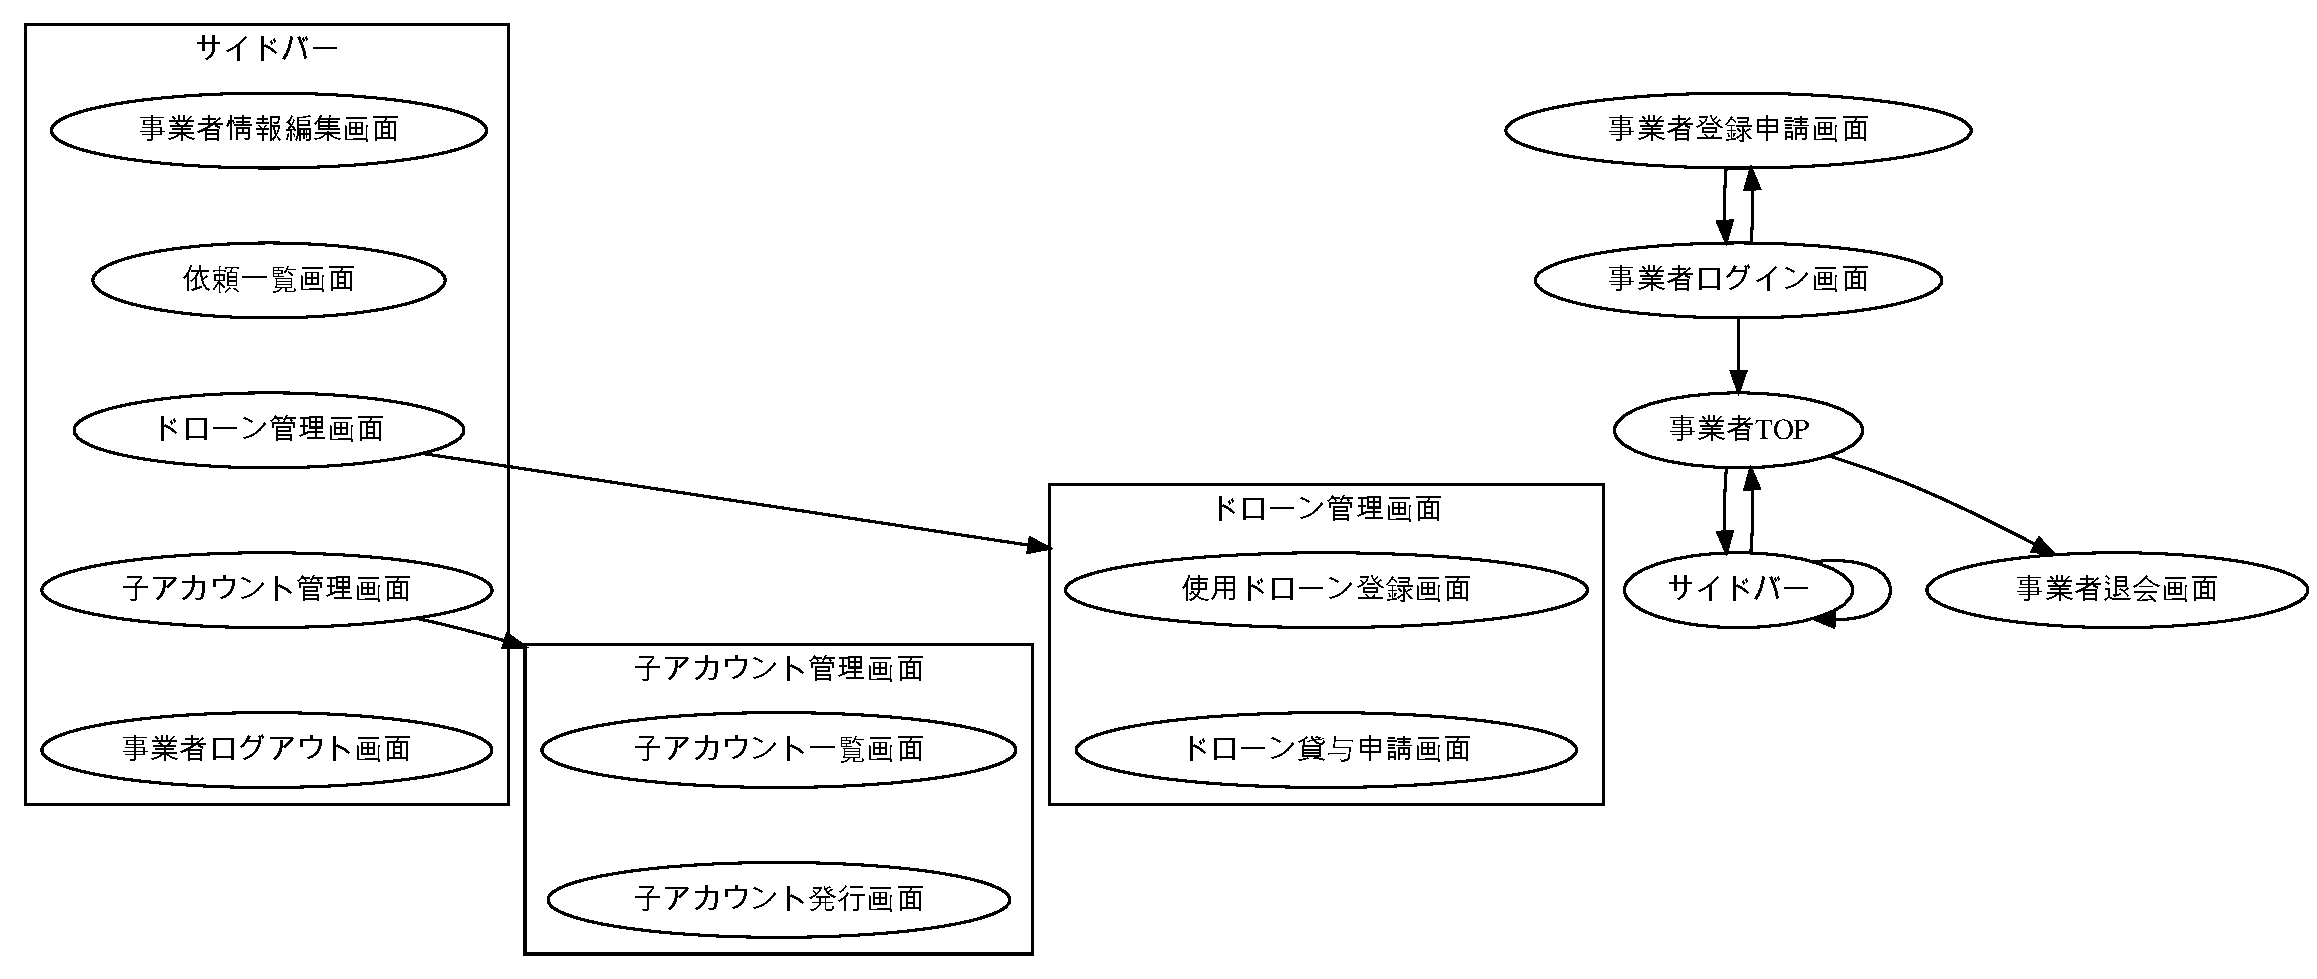
\includegraphics[width=\linewidth]{other/coop.pdf}
  \caption{事業者用ソフトフェアの画面遷移図}
  \label{fig:coop_diagram}
\end{figure}

\begin{figure}[H]
  \centering
  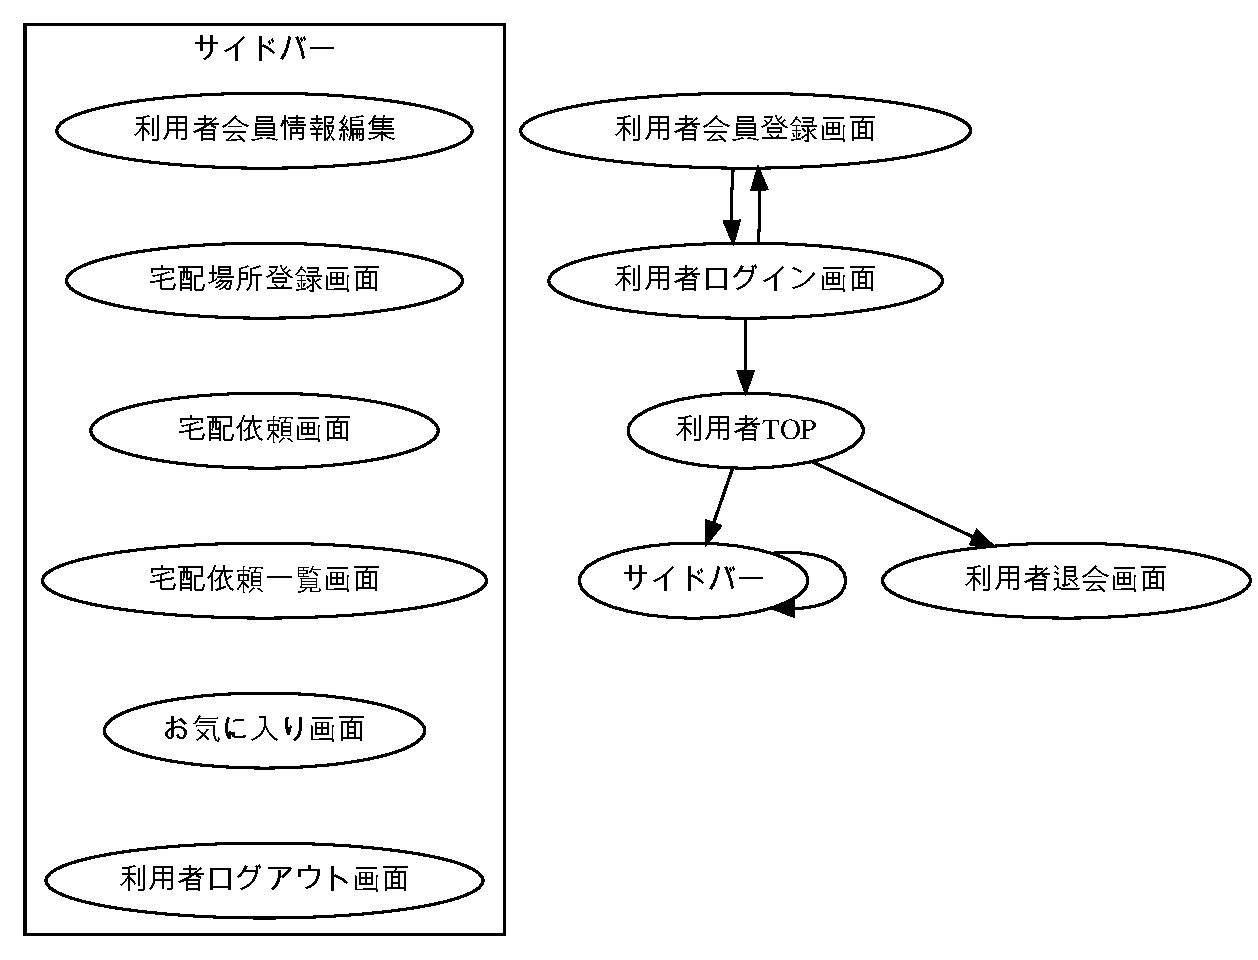
\includegraphics[width=\linewidth]{other/user.pdf}
  \caption{利用者用ソフトフェアの画面遷移図}
  \label{fig:user_diagram}
\end{figure}

\clearpage
\subsection{管理者向け画面}
以下に管理者向けの各機能に対する画面を示す.
\subsubsection{ログイン画面}
ログインすることで各機能を利用できる.
\ui{\detokenize{admin/admin_login_0.pdf}}{ログイン画面}
\ui{\detokenize{admin/admin_login_1.pdf}}{ログイン画面}
\clearpage
\subsubsection{ログアウト画面}
ログアウトは,画面右上部のアイコン横のボタンから可能である.
\ui{\detokenize{admin/admin_logout_0.pdf}}{ログアウト画面}
\ui{\detokenize{admin/admin_logout_1.pdf}}{ログアウト画面}
\clearpage
\subsubsection{事業者管理画面}
事業者管理画面では,事業者の地域別の絞り込みが可能である.
\ui{\detokenize{admin/admin_management_coop_0.pdf}}{事業者管理画面}
\ui{\detokenize{admin/admin_management_coop_1.pdf}}{事業者管理画面}
\clearpage
\subsubsection{事業者情報詳細画面}
事業者情報詳細画面では,該当事業者の詳細情報を確認できる.
\ui{\detokenize{admin/admin_view_coop_info.pdf}}{事業者情報詳細画面}
\subsubsection{事業者支払い情報詳細画面}
事業者支払い情報詳細画面では,該当事業者の支払いに関する詳細情報を確認できる.
\ui{\detokenize{admin/admin_view_coop_payment.pdf}}{事業者支払い情報詳細画面}
\clearpage
\subsubsection{事業者支払い情報編集画面}
事業者支払い情報編集画面では,該当事業者の支払いに関する情報を編集できる.
\ui{\detokenize{admin/admin_edit_coop_payment_0.pdf}}{事業者支払い情報編集画面}
\ui{\detokenize{admin/admin_edit_coop_payment_1.pdf}}{事業者支払い情報編集画面}
\clearpage
\subsubsection{ドローン貸与申請一覧画面}
ドローン貸与申請一覧画面画面では,事業者からの貸与申請の確認及び編集が出来る.
\ui{\detokenize{admin/admin_drone_loan_request_list.pdf}}{ドローン貸与申請一覧画面}
\clearpage
\subsubsection{貸与ドローン管理画面}
貸与ドローン管理画面では,貸与したドローンの管理が出来る.
\ui{\detokenize{admin/admin_management_coop_drone_0.pdf}}{貸与ドローン管理画面}
\ui{\detokenize{admin/admin_management_coop_drone_1.pdf}}{貸与ドローン管理画面}
\clearpage
\subsubsection{利用者管理画面}
利用者管理画面では,利用者の地域別の絞り込みが可能である.
\ui{\detokenize{admin/admin_management_user_info_0.pdf}}{利用者管理画面}
\ui{\detokenize{admin/admin_management_user_info_1.pdf}}{利用者管理画面}
\clearpage
\subsubsection{利用者情報詳細画面}
利用者情報詳細画面では,該当利用者の詳細情報を確認できる.
\ui{\detokenize{admin/admin_management_user_detail.pdf}}{利用者情報詳細画面}
\clearpage
\subsubsection{事業者情報分析画面}
事業者情報分析画面では,事業者情報を表またはグラフにて分析できる.
\ui{\detokenize{admin/admin_view_coop_statistics_0.pdf}}{事業者情報分析画面}
\ui{\detokenize{admin/admin_view_coop_statistics_1.pdf}}{事業者情報分析画面}
\clearpage
\subsubsection{利用者情報分析画面}
利用者情報分析画面では,利用者情報を表またはグラフにて分析できる.
\ui{\detokenize{admin/admin_view_user_statistics_0.pdf}}{利用者情報分析画面}
\ui{\detokenize{admin/admin_view_user_statistics_1.pdf}}{利用者情報分析画面}
\clearpage
\subsubsection{宅配依頼一覧画面}
宅配依頼一覧画面では,宅配依頼を確認することが出来る.
\ui{\detokenize{admin/admin_delivery_request_list.pdf}}{宅配依頼一覧画面}
\clearpage

\subsection{事業者向け画面}
以下に事業者向けの各機能に対する画面を示す.
\subsubsection{ログイン画面}
ログインすることで各機能を利用できる.
\ui{\detokenize{coop/coop_login_0.pdf}}{ログイン画面}
\ui{\detokenize{coop/coop_login_1.pdf}}{ログイン画面}
\clearpage
\subsubsection{ログアウト画面}
ログアウトは,画面右上部のアイコン横のボタンから可能である.
\ui{\detokenize{coop/coop_logout_0.pdf}}{ログアウト画面}
\ui{\detokenize{coop/coop_logout_1.pdf}}{ログアウト画面}
\clearpage
\subsubsection{事業者登録申請画面}
本画面にて事業者としての申請を行うことができる.
\ui{\detokenize{coop/coop_registration_request_0.pdf}}{事業者登録申請画面}
\ui{\detokenize{coop/coop_registration_request_1.pdf}}{事業者登録申請画面}
\clearpage
\subsubsection{事業者情報編集画面}
事業者情報編集画面では,事業者情報の更新が可能である.
\ui{\detokenize{coop/coop_edit_coop_info_0.pdf}}{事業者情報編集画面}
\ui{\detokenize{coop/coop_edit_coop_info_1.pdf}}{事業者情報編集画面}
\clearpage
\subsubsection{宅配依頼一覧画面}
宅配依頼一覧画面では,担当する宅配依頼の選択等を決定できる.
\ui{\detokenize{coop/coop_delivery_request_list.pdf}}{宅配依頼一覧画面}
\subsubsection{所持ドローン一覧画面}
所持ドローン一覧画面では,自身の保有するドローンを確認できる.
\ui{\detokenize{coop/coop_drone_list.pdf}}{所持ドローン一覧画面}
\clearpage
\subsubsection{ドローン登録画面}
ドローン登録画面では,貸与されたドローン以外のドローンを登録できる.
\ui{\detokenize{coop/coop_drone_registration.pdf}}{ドローン登録画面}
\subsubsection{子アカウント作成画面}
子アカウント作成画面では,同一事業者内で利用可能な子アカウントの作成を行える.
\ui{\detokenize{coop/coop_create_child_account.pdf}}{子アカウント作成画面}
\clearpage
\subsubsection{子アカウント一覧画面}
子アカウント一覧画面では,子アカウントの確認を行うことが出来る.
\ui{\detokenize{coop/coop_child_account_list.pdf}}{子アカウント一覧画面}
\subsubsection{ドローン貸与申請画面}
ドローン貸与申請画面では,ドローンの貸出を申請することが出来る.
\ui{\detokenize{coop/coop_drone_lent_request.pdf}}{ドローン貸与申請画面}
\clearpage
\subsubsection{退会画面}
退会画面は,画面右上部のアイコン横のボタンから可能である.
\ui{\detokenize{coop/coop_withdraw_0.pdf}}{退会画面}
\ui{\detokenize{coop/coop_withdraw_1.pdf}}{退会画面}
\ui{\detokenize{coop/coop_withdraw_2.pdf}}{退会画面}
\clearpage

\subsection{利用者向け画面}


\section{運用・保守設計}
本システムはAWSで構築することを前提とする,基本的には24時間365日システムを稼働させる.
% 従って24時間365日という時間はオンライン/バッチを含みシステムが稼働している時間として定義する.
ただし,毎月頭の深夜1時間程度メンテナンスの為にシステムを停止させる.
\subsection{運用設計}
% ここ調べないと分からない.
基本的にはDBのみ一定時間ごとにRDSがバックアップを取る.
それ以外のサーバについてはコンテナを用いて素早い復旧を可能にする.
% 各種サーバはDockerか何かですぐに立ち上がるようにする.
% 具体的なやつはAWSの機能を調べたら良いらしい.

\subsection{保守設計}
保守設計はシステムに変更を加えてシステムを維持することを目的とする.
% (先輩の資料が何を言ってるのかよく分からん)
システムログと管理者からの報告からバグをリストアップした後,ドキュメント化し開発環境にて修正を行う.
システムアップデートについても開発環境にて検証を行う.
バグの修正とシステムアップデートは致命的なもの以外は毎月のメンテナンスにて反映する.
緊急性の高いものは開発環境で動作確認を終えた後,迅速に緊急メンテナンスを行い反映する.
\clearpage
\section{データベース設計}
本システムのデータベース設計を図\ref{fig:database}に示す.
主キーを PK,外部キーを FK として記載している.
\begin{figure}[H]
  \centering
  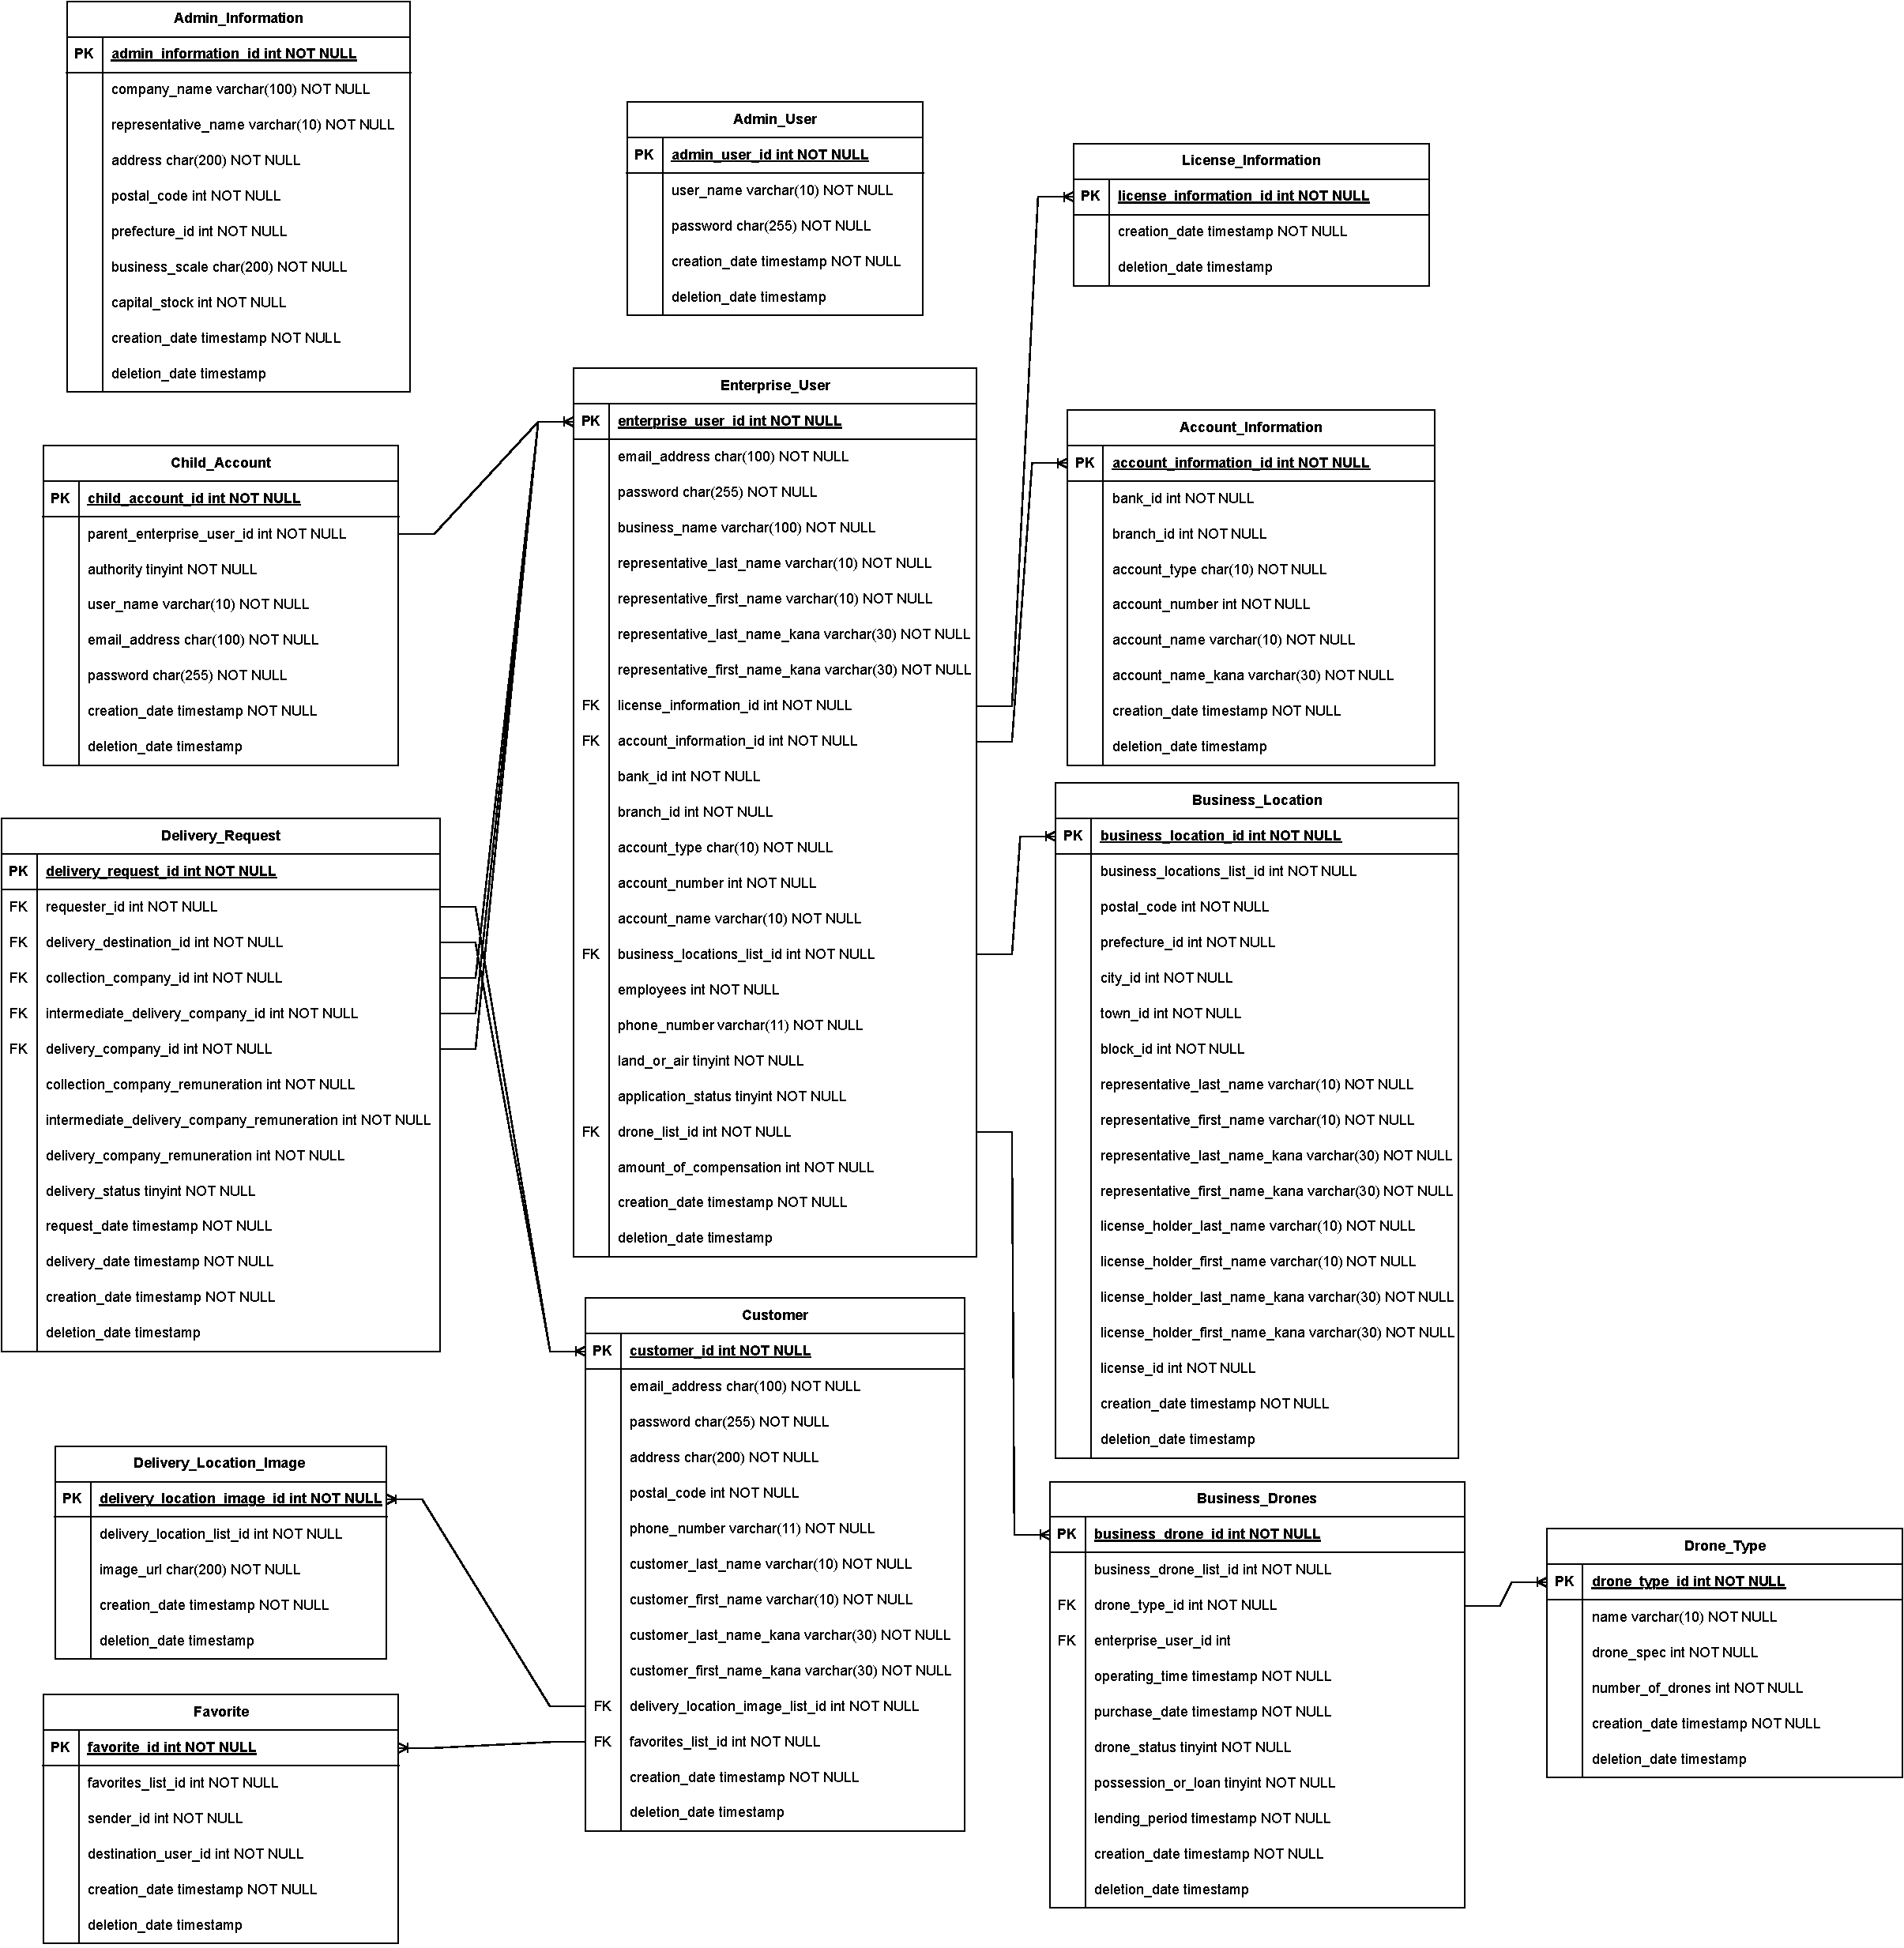
\includegraphics[width=\textwidth]{other/database.pdf}
  \caption{データベース}
  \label{fig:database}
\end{figure}

\clearpage
\section{ネットワーク設計}
図\ref{fig:network}は,本システムのネットワーク構成を示したものである.
本システムは,Amazon Web Services(AWS) の Amazon Cloud Front を用いて作成する.
Amazon Virtual Private Cloud(Amazon VPC) を用い,2つのアベイラビリティゾーン間でのトラフィックの共有を行う.

インターネットゲートウェイにより,各アベイラビリティゾーンへと通信を分散させ,サーバと管理者・事業者・利用者がそれぞれ通信を行う.
各アベイラビリティゾーン内では,Amazon Elastic Compute Cloud(EC2) 及び Amazon Relational Database Service(RDS) インスタンスを構築し,EC2インスタンスがリクエストの処理及びデータベースとの通信を行う.

上記の構成要素の手前で,AWS WAF を利用しセキュリティの対策を行う.

\begin{figure}[H]
  \centering
  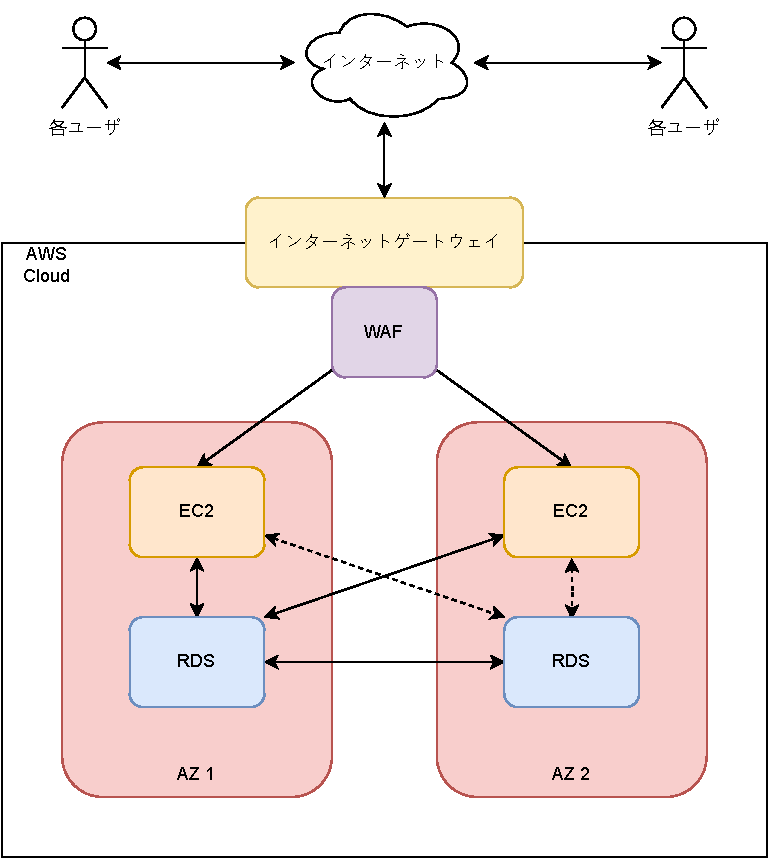
\includegraphics[width=0.8\textwidth]{./other/network_img.pdf}
  \caption{ネットワーク構成図}
  \label{fig:network}
\end{figure}

\section{非機能要件}
本システムが保証する非機能要件は以下の通りである.
\subsection{セキュリティ対策}
本システムでは以下のセキュリティ対策を行う.
\subsubsection{ファイアウォール}
サーバーとの通信時にAWS WAFを用いてファイアウォールを作成し不正アクセスのリスクを軽減する.
\subsubsection{権限設定}
開発・運用・保守時に適切な権限を設定することで不正アクセスされた際のリスクを軽減する.
\subsubsection{通信の暗号化}
ユーザーが本システムにアクセスする際の通信をSSL/TLSを用いて暗号化することで,通信内容の盗聴のリスクを軽減する.
\subsubsection{データベースの暗号化}
データベースに保存されるインスタンスをAWS KMS keyを用いて暗号化することで,不正アクセスされた際のリスクを軽減する.
\subsubsection{パスワードのハッシュ化}
ハッシュ化されたパスワードをデータベースに保存することで,不正アクセスによるパスワード流出のリスクを軽減する.
\subsubsection{DDoS攻撃対策}
DDoS攻撃の対策としてAWS Shieldを用いる.
\subsection{障害対策}
本システムでは以下の障害対策を行う.
\subsubsection{サーバーの冗長化}
データベースサーバーに対して可用性向上の為,プライマリ・セカンダリ構成の冗長化を行う.
\subsubsection{サーバーの負荷分散}
特定のwebサーバーに対して負荷が集中することを避けるために,ロードバランサーを用い負荷の分散を行う.

\section{貢献度}
\begin{itemize}
  \item 1240312 久保田 天治 : 非機能要件の設計及びフロー図,UI図の作成.
  \item 1250329 塩澤 康志 : データベース設計及びフロー図,UI図の作成 週当番としての職務を果たした.
  \item 1250333 蝉 祐介 : フロー図,UI図の作成 週当番としての職務を果たした.
  \item 1250348 寺内 俊輔 : テンプレートの作成及びフロー図の作成 チームのバランスを確保(仲裁) タスク表を作成及び管理.
  \item 1250358 林 晃太郎 : UIの画面遷移図の作成及びフロー図,UI図の作成.
  \item 1250371 松本 吏司 : ネットワーク設計及びフロー図,UI図の作成 作業用リポジトリの整備 週当番としての職務を果たした.
\end{itemize}
\bibliographystyle{junsrt}
\bibliography{References.bib}
\end{document}
